\section{Le jeu de rôle, un conte interactif}

\begin{figure}[h!]
    \centering
    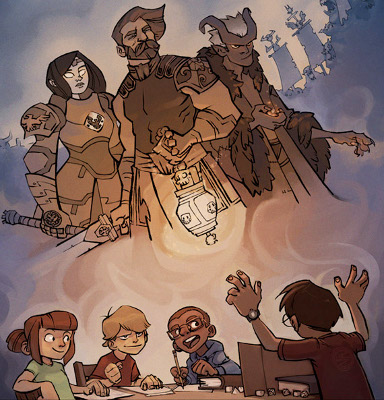
\includegraphics[width=0.80\linewidth]{img/rpg_tabletop2.jpg}
    \caption{Tabletop RPG}
\end{figure}


\subsection{Des objectifs antagoniques}

\begin{shadequote}
Un peuple, c'est une population, plus des contours et des conteurs. \par\emph{Régis Debray, Éloge des frontières}
\end{shadequote}

Conceptualisés en des temps forts éloignés, les visées des contes et jeux de rôles \textit{sur table} sont fondamentalement opposés. Si le premier voue son existence à la transmission d'une expérience et au renouvellement d'une tradition ancestrale, le second est porteur d'intentions plus légères, favorisant la simulation d'une expérience exaltante pour le plaisir du joueur. La profondeur du message transmis diffère donc grandement, de même que l'ancrage au monde réel de l'histoire.

Si certaines licences sont permises au conte afin d'enjoliver son récit, le jeu de rôle s'affranchit volontairement du réel, n'hésitant pas à décrire un univers fictif aux êtres et paysages de légende afin de stimuler l'imagination et l'émerveillement de son auditoire.

La nature interactive du jeu de rôle doit également être mentionnée, le bon déroulement du scénario proposé étant fonction des réactions de ses joueurs. Dans le cas d'un conte, la nature de vécu du récit narré restreint les possibilités d'adaptation, la conformité au possible devant primer et l'auditoire respectant une certaine passivité.

On notera enfin la disproportion des processus d'immersion et d'identification entre ces pratiques, la profondeur addictive permise dans le cadre du jeu de rôle résultat notamment de l'attache sentimentale du joueur au protagoniste à son image et d'une pratique abusive de ces jeux. Cette addiction pouvant donner lieu à un renfermement sur une communauté restreinte de \textit{rolistes\footnote{Roliste : joueur de jeu de rôle}}, on tendra donc à rapprocher les jeux de rôles aux jeux virtuels éponymes, loin des contes traditionnels.



\subsection{Une portée analogue}

\begin{shadequote}
L'art de raconter des histoires est toujours l'art de reprendre celles que l'on a entendues. \par\emph{Walter Benjamin, Der Erzähler}
\end{shadequote}


Si certaines dissemblances peuvent être naturellement observées entre contes et jeux de rôles, une forme homologue à ces pratiques doit néanmoins être notée. Il s'agît en effet là de procédés de nature sociale, tendant à rapprocher les êtres autour d'une expérience commune. Aux antipodes des es récits oraux narrés par un conteur ou un \textit{maître du jeu} visent à transporter leur auditoire dans un environnement dont la représentation est laissée libre à chacun, une ambiance soignée et une imagination fertile étant les clefs d'une immersion réussie. La démarcation avec le domaine du jeu virtuel se ressent donc notamment par l'absence de l'écran, importante frontière sociale, et le rôle prépondérant de l'imaginaire.

Si conteur et \textit{maître du jeu} tendent en outre à concentrer les rôles de leurs protagonistes, la dimension sociale du jeu de rôle se voit renforcée par une délégation de certains d'entre-eux accompagnée de dialogues animés entre joueurs.\\


Par ailleurs, le \textit{maître du jeu} se devant de réagir aux décisions prises par ses joueurs afin de maintenir une trame d'histoire cohérente, il lui incombe la responsabilité subtile d'orienter les interactions des joueurs dans le sens du scénario préparé. Malgré de perpétuelles et inévitables retouches, l'objectif est alors de faire croire au joueur que ses actions ont un impact profond sur l'aventure vécue, alors qu'il s'agît plus souvent de descriptions, jeux de scènes et dialogues visant essentiellement à favoriser son immersion. Des retournements de situation et références aux actions passées mesurés auront donc pour but de simuler l'interactivité plus que de s'y adapter.

Ces légères retouches coïncident de surcroît avec celles apportées par le conteur à son récit, élaborant ainsi des versions successives de son histoire en fonction des réactions du public. Un conte s'étaye donc au fil de ses représentations, l'étude du public associée à un dialogue une fois la séance terminée permettant de déceler et corriger les imperfections du conte.\\


On constatera finalement les convergence thérapeutiques de ces pratiques, lesquelles par l'exercice de la \textit{catharsis} libèrent l'auditoire de ses pulsions. Étendant les vertus des contes, les jeux de rôles iront jusqu'à affermir la confiance en soi de l'auditoire, lui permettant de se découvrir, et de progressivement se construire.

\clearpage
